\section{Planlægning}

Vi holdt ugentlige møder med fast mødetidspunkt. Vi lavede aftaler omkring deadlines på de enkelte møder, og sørgede for at blive færdige med de enkelte opgaver til de aftalte tider. Fra møde til møde opdaterede vi hinanden i forhold til status på opgaver. Vi henviste yderligere til vores projektopgavetavle ved møderne for udspecificeret status på f.eks ”in progress”-posten. (Se figur \ref{fig:SB})  
 I begyndelsen af processen lavede Victor et Gannt-diagram. Det var dog ikke noget vi benyttede fremefter grundet overgangen til brug af arbejdsopgave-boardet og sprint, men det gav et godt overblik over opgavens omfang i begyndelsen af semesteret. Denne tidsplan i fuldendt såvel som review indelt kan findes under Bilag/Værktøjer og har filtyben .gan. 
Større projektmæssige deadlines i forhold til reviews og aflevering blev skrevet op med stor og tyk skrift og hængt op på den midterste og mest centrale tavle i vores grupperum. 
Yderligere har Kimmie stået for at sørge for at vores mødelokale har været fast booket.

% Scrum Board
\begin{figure}[H] \centering
    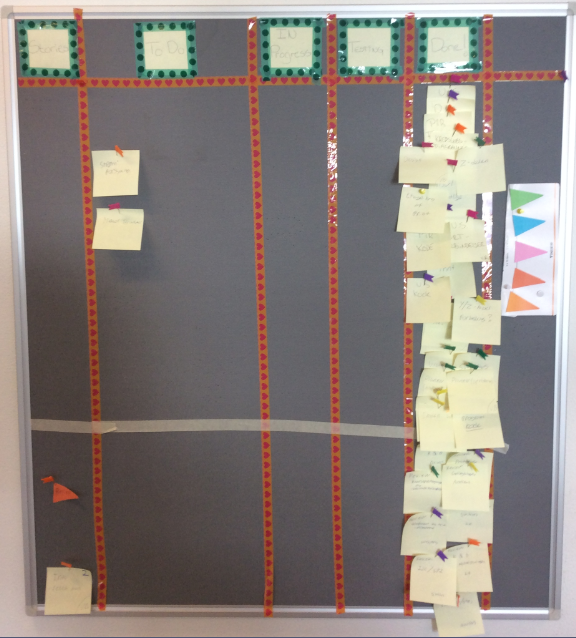
\includegraphics[width=0.5\textwidth]{0_Filer/ScrumBoard.PNG}
    \caption{Projektopgavetavle}
    \label{fig:SB}
\end{figure}
